\chapter{Detecção de Intrusão em um Cenário Real} \label{ch:cenário-real}
 %- Em cada capitulo adicionar um texto introdutório

Este capítulo esta organizado da seguinte forma: A próxima seção apresenta o cenário de testes, descrevendo características gerais da rede selecionada para os teste. Na seção \ref{sec:infraestrutura} será abordado a infraestrutura usada para os testes, ferramentas utilizadas e as configurações feitas. Na seção \ref{sec:testes} será descrito os testes realizados com suas respectivas justificativas. Na seção \ref{sec:resultados} será apresentado os resultados esperados e obtidos, problemas encontrados e a comparação das ferramentas e por último, na seção \ref{sec:conclusão}, uma breve conclusão.

\section{Metodologia dos Testes}

Nessa seção será descrito o cenário utilizado para a realização dos testes. Na \autoref{sec:cenário}, aborta a rede onde os sensores foram instalados e algumas de suas estatísticas de uso. A \autoref{sec:infraestrutura} descreve a infraestrutura montada para realização dos testes, os equipamentos utilizados e as ferramentas adicionais. Na \autoref{sec:testes}, será descrito os testes realizados. Na \autoref{sec:resultados} abordará os resultados esperados e obtidos com os testes. Por último, na \autoref{sec:conclusão} a conclusão.

% (Adicionar o escopo dos testes): descrever o ambientes,
\subsection{Cenário de Testes} \label{sec:cenário}

\begin{figure}[!htb]
\centering
\caption{Tráfego da Rede de Teste}
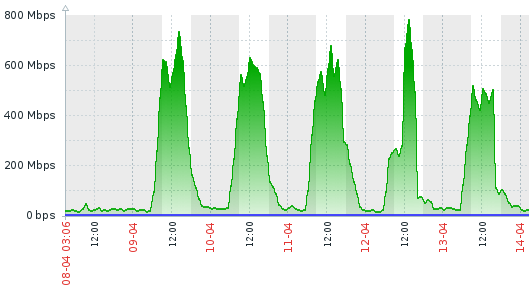
\includegraphics[scale=.7]{trafego-rede.png}
\label{fig:trafego-rede}
\legend{Fonte: \cite{zabbix}}
\end{figure}

%Descrever o cenário. Ex: Uma rede com XXX usuários; Os usuários utilizam
%diferentes ferramentas,...
%Adicionar gráficos de utilização da rede

\subsection{Infraestrutura Definida para Testes} \label{sec:infraestrutura}
%Descrever o que foi utilizado:
%Ex: Equipamentos - Servidores, ....
%    Configuração
%    Ferramentas - Snort (referenciar capítulo), ...

No ambiente de teste foi usado uma máquina Dell com 134 Megabytes (MB) de memória RAM e 40 núcleos. Usou-se XenServer \cite{xenserver} versão 7, sistema operacional (SO) \textit{opensource} da Citrix voltado para virtualização. Foram testados outros SOs porém somente o XenServer possuía, na época da instalação do ambiente, \textit{firmware} da placa de rede do \textit{host} compatível e que funcionava com instabilidade. 
 
Outro fator que pesou na escolha do SO foi a experiência com a plataforma e por existir uma interface para gerencia chamada XenCenter que roda no Windows. Uma alternativa \textit{opensource} desse software é o OpenXenManager que funciona nos sistemas Unix \cite{openxenmanager}.

No primeiro momento, foi instalado uma máquina virtual com o sistema operacional Debian 9.3 \textit{codename} Stretch \cite{debianwheezy}, uma distribuição linux com uma proposta de ser totalmente livre, usada como base para instalação de outras máquinas utilizando o recurso de \textit{snapshot}, uma cópia de uma máquina virtual rodando em um certo momento, do XenServer. O uso desse recurso foi necessário para criar um ambiente igual para as ferramentas em estudo.

Foi alocado 8 MB memória RAM, 4 processadores e 100 Gigabytes(GB) de espaço em disco para o \textit{snapshot}. Esses valores foram definidos com base em um estudo \cite{mikelococo} que considera vários fatores, como largura da rede, localização do IDS e versão, tipo do capturador de tráfego e tamanho da base de assinaturas para dimensionar os recursos de memória e processamento, aplicado especificamente ao Snort. A mesma regra foi aplicada ao Suricata.

Para o \textit{host} conseguir pegar o pacotes destinados a rede escolhida para o experimento, foi necessário uma configuração de espelhamento no roteador B (Figura \ref{fig:infra-ambiente}) que consiste na copia dos pacotes que saem pela porta dessa rede no roteador para a porta conectada no \textit{host} que possui uma largura de banda de 10 Gigabits. A interface de rede do \textit{host} precisou ser configurada no modo \textit{promisc}.

Posteriormente criou-se três máquinas virtuais, duas usadas para instalação dos IDSs (Suricata e Snort) e a terceira será usada para rodar o \textit{framework} Pytbull (\autoref{sec:pytbull}). Numa quarta máquina, instalou-se o sistema Kali Linux \cite{kalilinux} para geração de ataques, esse SO possui ferramentas nativas para testes de penetração e auditoria de segurança (Metasploit \autoref{sec:metasploit}, NMAP \autoref{sec:nmap} e OpenVAS \autoref{sec:openvas}). A infraestrutura final do ambiente de teste poder ser visualizada na \autoref{fig:infra-ambiente}.

\begin{figure}[!htb]
\centering
\caption{Infraestrutura do ambiente de teste}
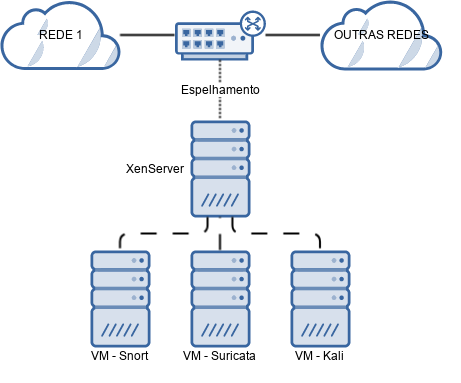
\includegraphics[scale=.65]{infra.png}
\label{fig:infra-ambiente}
\legend{Fonte: Autoria própria}
\end{figure}

Para coleta das informações de uso de recurso de hardware como memória, processamento e I/O das máquinas com os IDSs utilizou-se o \textit{daemon} Collectd \cite{collectd}. Outra opção para essa finalidade é a utilização de um servidor de monitoramento como o Zabbix \cite{zabbix}. A ideia de ter duas ferramentas para essa analise é fazer um comparativo e validar as informações coletadas.

O formato usado para facilitar a análise do \textit{logs} foi JavaScript Object Notation (JSON), um formato simples, leve e de fácil leitura. O Motor de Saída do Suricata já tem suporte a esse tipo de formato o que não acontece no Snort. Para tal, usou-se o IDSTools \cite{py-idstools}, uma coleção de bibliotecas na linguagem python que trabalha para auxiliar o IDS Snort. Dentre os utilitários presentes nessa coleção, temos o idstools-u2json, que converte, de forma continua, arquivo no formato unified2, uma das saídas disponível no Snort, para o formato JSON.

Para analisar os \textit{logs}, usou-se uma infraestrutura que combina três ferramentas:

\begin{alineas}
\item \textbf{Kibana} \cite{kibana}: Uma plataforma de análise e visualização desenhada para trabalhar com os índices do Elasticsearch \cite{elasticsearch}, a grosso modo, podemos dizer que ela é uma interface gráfica para o Elasticsearch. 
\item \textbf{Elasticsearch}: Um motor de busca e análise altamente escalável, capaz de armazenar, buscar e analisar uma grande quantidade de dados em tempo próximo ao real. 
\item \textbf{Logstach} \cite{logstach}: Um motor de coleta de dados em tempo real, unificando os dados de diferentes fontes dinamicamente, normalizando-os nos destinos escolhidos.
\end{alineas}

Dessa forma centralizou-se os \textit{logs}, facilitando a visualização e analise das ocorrências geradas pelos IDSs. 

\section{Testes Realizados} \label{sec:testes}
%Quais os testes realizados com justificativa ?
%Descrição dos testes. Quais os testes foram realizados ?
Os testes realizados são simulações de passos que uma pessoa má-intencionada iria tomar para alguma tentativa de invasão, entende-se por invasão, qualquer tipo de violação e alteração não autorizada de um serviço ou \textit{host}.

O passo inicial seria um estudo do alvo utilizando várias técnicas mas principalmente a engenharia social, analisando as pessoas que trabalharam na organização, enviando spam e \textit{phishing} na tentativa de capturar dados como senhas de acesso. 

Posteriormente, o atacante iria observar o tráfego da rede, verificando os serviços que o alvo oferece, a procura de alguma senha desprotegida (não criptografada). Esse passo inicial não será aplicados nos testes pois seria impossível o IDS detectar.

O passo seguinte seria uma garimpagem de informações e mapeamento da rede, a procura de um \textit{host} vulnerável. A ferramenta escolhida para essa finalidade é o Nmap (\autoref{sec:nmap}). 

No primeiro teste de \textit{scan}, usou-se o parâmetro '-F', habilitando a modo \textit{fast} do Nmap. Nesse modo, são verificadas apenas as portas especificadas no arquivo nmap-services, que, na instalação padrão, possui 27372 portas descritas. Isso é muito mais rápido que verificar todas as 65535 portas tcp e 65535 portas udp, possíveis em um \textit{host}. Abaixo segue o comando usado.

\begin{lstlisting}[caption={Comando NMAP no modo \textit{fast}},language=bash, frame=single, label={lst:nmap-F}]
    nmap -F 200.239.72.19
\end{lstlisting}

O segundo teste, usou-se o parâmetro '-A' do NMAP. Essa opção habilita opções adicionais avançadas e agressivas, descobrindo versões dos serviço, determinando protocolos de serviços, o nome da aplicação, o número da versão, o nome do \textit{host} (utilizando o DNS reverso), tipo de dispositivo, sistema operacional, entre outras informações. Ter um número de versão exacto ajuda substancialmente na determinação de quais \textit{exploits} o servidor está vulnerável \cite{nmap}.

\begin{lstlisting}[caption={Comando NMAP no modo de descoberta de versões},language=bash, frame=single, label={lst:nmap-sv}]  
    nmap -A 200.239.72.19
\end{lstlisting}

Uma forma encontrada para automatizar o processo de execução dos comandos citados acima foi a criação de um código em \textit{shell script}. O \textit{Shell Script} é uma linguagem de script usada por vários sistemas operacional, principalmente os baseados em UNIX. Abaixo segue o código.

\begin{lstlisting}[caption={Automatização das execuções do comando NMAP},language=bash, frame=single, label={lst:script-nmap}]
#!/bin/bash

echo "\nIniciando ..."
STARTIME=$(date)

for i in $(seq 1 100)
    do  
        echo "\n$i Execução..."
        nmap $1 200.239.72.19 > /dev/null
        sleep 5
    done

ENDTIME=$(date)                                                                                                                                                                 
echo "\nInicio $STARTIME"
echo "\nFim $ENDTIME"
\end{lstlisting}

Na primeira linha de um código em \textit{shell script}, precisamos especificar o interpretador utilizado (\#!/bin/bash). Criou-se duas variáveis, uma para armazenar a hora do inicio do \textit{script} e uma para armazenar termino, dessa forma, a pesquisa pelos alertas gerados pelas ferramentas será menos dispendiosa. O comando NMAP foi colocado dentro de um laço \textit{for}, executado 100 vezes. 

De posse de um alvo em potencial, próximo passo seria rodar um \textit{scanner} de vulnerabilidade, em busca de brejas já conhecidas, e que, geralmente por descuido do administrador, não foi fechada. Essas brejas podem ter várias origens, desde uma versão do serviço com \textit{bugs} ou uma má configuração. Para esse teste, usou-se o OpenVAS (\autoref{sec:openvas}).

É necessário algumas configurações no \textit{scanner} nessa etapa. Primeiramente, deve-se definir o alvo, tal configuração é feita através do caminho "\textit{Configuration > New target}", a \autoref{fig:openvas-newtarget} mostra a janela aberta, nela temos que definir um nome para o alvo e o IP ou a faixa de IP's, as outras configurações serão deixadas com o padrão.

\begin{figure}[!htb]
\centering
\caption{Definição do alvo no OpenVAS}
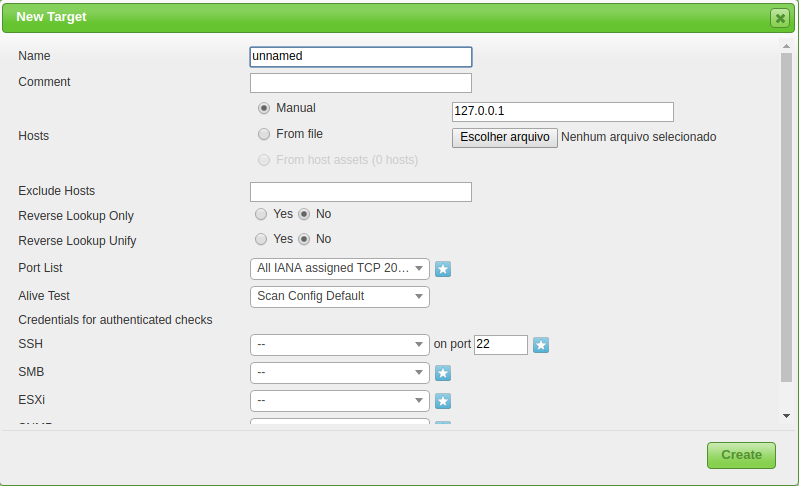
\includegraphics[scale=.55]{openvas-newtarget.png}
\label{fig:openvas-newtarget}
\legend{Fonte: Autoria própria}
\end{figure}

A realização do scan é feita através do caminho "\textit{Scans > Tasks > New Task}", na \autoref{fig:openvas-newtask} mostra a janela aberta, nela precisamos definir no nome da \textit{task} e o alvo, que foi definido anteriormente, as outras opções serão deixadas com o padrão. 

Por padrão, quando uma \textit{task} é criada, o \textit{scan} é automaticamente executado. Esse processo pode demorar, isso depende de quantos alvos foram definidos. Ao final, um relatório é exibido com as vulnerabilidades encontradas e categorizadas (\textit{high, medium, low}) de acordo com a sua severidade. Além disso, o OpenVAS exibe um sumário, descrevendo a(s) falha(s) encontrada(s) e como resolver ou mitigar o problema.

\begin{figure}[!htb]
\centering
\caption{Configuração de um \textit{task} de scan no OpenVAS}
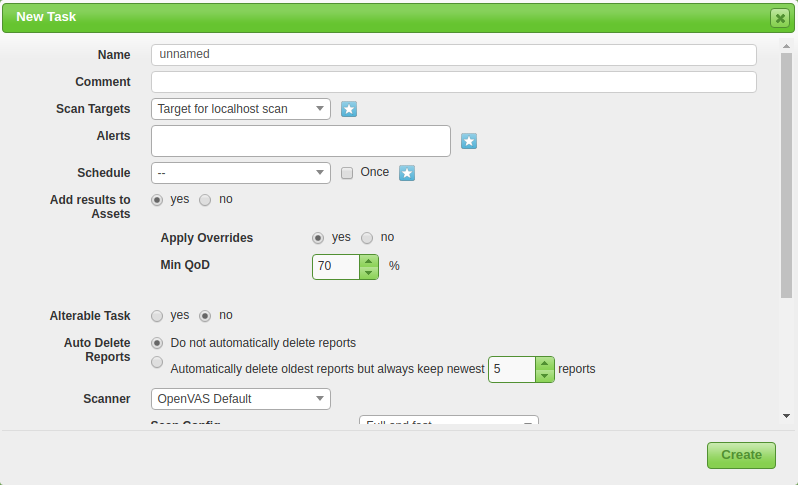
\includegraphics[scale=.55]{openvas-newtask.png}
\label{fig:openvas-newtask}
\legend{Fonte: Autoria própria}
\end{figure}

Outro teste realizado determinará a capacidade das ferramentas de detectar ataques de negação de serviço (\autoref{sec:negação}). Existem várias técnicas para realizar esse tipo de ataque, o usado nesse trabalho foi o TCP SYN FLOOD. 

Quando um cliente tenta começar um conexão TCP com um servidor, são trocados, entre eles, uma série de mensagens (\textit{Three-Way Handshaker}). O TCP SYN FLOOD consiste em enviar uma sequência de requisições SYN para o alvo, sobrecarregando-o diretamente na camada de transporte e indiretamente na camada de aplicação.

Para tal, usou-se o Metasploit Framework (\autoref{sec:metasploit}). Primeiramente, entrou-se no console de linha de comando, para acessar, basta, no terminal, digitar \textit{msfconsole}. Existe um modulo no Metasploit chamado \textit{synflood}, para utilizar esse modulo, é necessário definir o IP do alvo e o IP de onde partirá o ataque. Abaixo segue os comandos usados no \textit{msfconsole}.

\begin{lstlisting}[caption={Comando usados no Metasploit para ataque de negação de serviço},language=bash, frame=single, label={lst:synflood}]
use auxiliary/dos/tcp/synflood

msf auxiliary(synflood) > set rhost 200.239.72.19 (target IP)

msf auxiliary(synflood) > set shost 10.15.10.20 (attack IP)

msf auxiliary(synflood) > exploit
\end{lstlisting}

No ultimo teste, utilizou-se o \textit{framework} Pytbull (\autoref{sec:pytbull}). O Pytbull foi desenvolvido especificamente para realizar testes e validar configurações em IDPS. A documentação oficial exemplifica algumas arquiteturas que podem ser usadas, nesse trabalho usou-se a arquitetura \textit{remote mode} onde o IDS é colocado para escutar todo o tráfego que passa no \textit{switch} através de uma porta espelhada e com uma interface configurada em modo \textit{promisc}.

Por padrão, todos os testes do \textit{framework} estão ativados. Como o teste de DoS foi realizado utilizando o Metasploit, e para diminuir o tempo da experimentação, o módulo denialOfService do Pytbull foi desativado. Outro módulo desativado, devido demora na execução, foi o testRules, a execução desse módulo levava mais de uma hora. Para desativar esses módulos precisa-se editar o arquivo \textbf{pytbull/config/config.cfg}, alterando, na parte dos testes, os valores de 1 para 0.

Outra mudança feita, somente nessa fase, com o intuito de melhorar a eficácia do teste, foi a configuração das ferramentas de IDPS para analisar somente pacotes com o IP do \textit{host} que executará o Pytbull. 

Antes de executar o \textit{framework}, é necessário mover, para os \textit{hosts} que estão executando as ferramentas de IDPS, o script \textbf{pytbull/server/pytbull-server.py} encontrado no arquivo .tar.bz2, baixado no site oficial do Pytbull \cite{pytbull}. Esse executável abre um shell reverso no servidor que é usado pelo módulo clientSideAttacks do Pytbull, fazendo-o baixar arquivos maliciosos da Internet. 

Feito isso, basta executar os comandos abaixo, substituindo \textbf{suricata} e \textbf{snort} pelos seus respectivos IPs:

\begin{lstlisting}[caption={Comandos usados para execução do Pytbull}, language=bash, frame=single, label={lst:pytbull}]
cd pytbull/

sudo ./pytbull -t suricata

sudo ./pytbull -t snort
\end{lstlisting}

\section{Resultados} \label{sec:resultados}
%Resultados esperados e obtidos
%Quais os resultados dos testes ??
%Comparação das ferramentas
%Problemas encontrados
O Snort e Suricata são Sistemas de Detecção de Intrusão baseados em assinaturas, ambos gratuitos e multiplataformas, no entanto, caso queira uma base de assinaturas robusta e com suporte, o mesmo deve ser adquirido mediante a um pagamento. 

Nada impede o desenvolvimento de uma base própria, no entanto, é necessário uma equipe altamente capacitada e dedicada para esse fim, visto que, diariamente, são lançados na rede novos ataques ou variações de ataques existentes, tornando a atualização da base de assinaturas um processo árduo e custoso.

O Snort encontra-se consolidado no mercado há vários anos e com muitas versões, já o Suricata surgiu em 2010 como um novo motor, com a tecnologia \texit{multithreading} (processa várias tarefas ao mesmo tempo), aproveitando o paradigma multinúcleos dos processadores. Por esse motivo, espera-se que o desempenho do Suricata seja superior ao do Snort.

Foram encontrados vários desafios durante o desenvolvimento desse trabalho. Dentre elas, destacam-se a dificuldade de encontrar material e experimentos referente ao Suricata, a documentação oficial do sistema é pobre de conteúdo, limitando-se ao básico de instalação e algumas particularidades de configuração. 

Outra dificuldade que se destaca foi com relação a configuração do cenário de teste, devido a alta complexidade e por requerer configurações em vários equipamento, no qual, em alguns casos, a gerência pertencia a terceiros. Depois de um tempo, observou-se que nem todos os pacotes da interface espelhada estava passando para as VM's, isso afetaria os resultados dos testes. Após análise, concluiu-se que era necessário uma configuração de espelhamento no \textit{openvswitch} (utilizado pelo XenServer) do \textit{host}. 

As métricas usadas para análise e comparação das ferramentas são a utilização dos recursos de \textit{hardware} (memória, processamento), taxa de detecção, independente de ser falso positivo e falso negativo. No primeiro momento, havia a ideia de comparar utilizando essa métrica, no entanto, devido a uma quantidade muito grande de alertas e devido a rede ser grande (vários clientes), essa comparação tornou-se inviável.

No primeiro experimento realizado, utilizando o NMAP no modo \textit{fast}, a execução do \textit{script} \autoref{lst:script-nmap}, gerou um total de 62 alertas, dos quais 100\% deles foram do Snort. o Snort teve um desempenho melhor pois ele foi capaz de detectar a execução do comando.

No segundo teste de varredura, utilizando o NMAP no modo no qual é possível identificar as versões dos serviços e até o SO do alvo, as ferramentas geraram, com a execução do \textit{script} (\autoref{lst:script-nmap}), um total de 210 alertas, desses, 106 (50.5\%) foi gerado pelo Suricata e 104 (49.5\%) pelo Snort. Nesse cenário, houve quase uma equidade na taxa de detecção. No geral, nesse experimento com NMAP, o Snort teve um desempenho melhor, pois conseguiu gerar alertas no primeiro teste.

Já no teste realizado usando um \textit{scan} de vulnerabilidade (\autoref{sec:openvas}), os IDPS's geraram um total de 3071 alertas, sendo que 2142 (69.74\%) veio do Suricata e 929 (30.26\%) do Snort. Aqui, houve uma disparidade grande na taxa de detecção, assim, nesse cenário, o Suricata apresentou um desempenho melhor.

Para determinar se os IDPS's tinham capacidade de identificar ataques de negação de serviço utilizou-se um módulo do \textit{Metasploit Framework} (\autoref{lst:synflood}). Nesse teste, nenhuma uma das ferramentas alertou sobre a execução desse tipo de ataque. 

Por último, temos o teste utilizando \textit{framework} Pytbull (\autoref{lst:pytbull}). Para melhorar os resultados, configurou-se os IDPS's para apenas gerar alertas de eventos relacionados ao \textit{host} alvo. O resultado mostrou que houve um igualdade na taxa de detecção total, no entanto, o Suricata mostrou-se superior pois a quantidade não detectado do Snort foi maior, 81\% contra 47\% do Suricata. Abaixo segue os resultados, o gráfico é fornecido pelo próprio Pytbull ao final da execução. 

\begin{figure}[!htb]
\centering
\caption{Resultado da execução do \textit{framework} Pytbull sobre o Suricata}
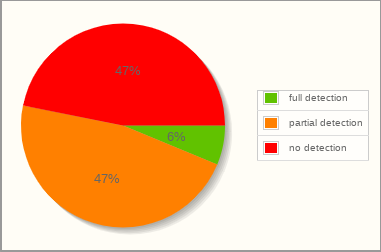
\includegraphics[scale=.7]{suricata-pytbull-report.png}
\label{fig:suricata-pytbull-report}
\legend{Fonte: Pytbull}
\end{figure}

\begin{figure}[!htb]
\centering
\caption{Resultado da execução do \textit{framework} Pytbull sobre o Snort}
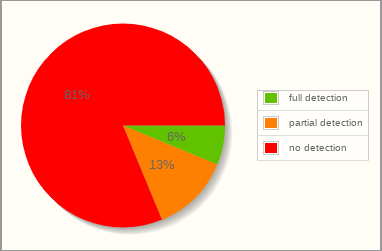
\includegraphics[scale=.7]{snort-pytbull-report.png}
\label{fig:snort-pytbull-report}
\legend{Fonte: Pytbull}
\end{figure}

Na \autoref{tab:suricata-recursos} está presente os dados coletados pelo serviço de monitoramento Zabbix do Suricata no decorrer de um mês. Foram coletados quatro informações, a carga do processador por núcleo nos tempos de um, cinco e quinze minutos e o uso de memória. Na \autoref{tab:snort-recursos}, há as mesmas informações, no entanto, do Snort.

Quanto a utilização de recurso de \textit{hardware}, conclui-se que o Snort utiliza um quantidade menor de memória, no entanto, possui um média de carga de processamento maior. Tal característica é válida devido a arquitetura do Snort usar apenas uma \textit{thread} por processo. O fato do processamento minimo do Suricata ser zero, dar-se a um comportamento da ferramenta, no qual o mesmo era finalizado de forma inesperada.  

\begin{table}[!htb]
\ABNTEXfontereduzida
\centering
\caption{Resultado do uso de recurso de \textit{hardware} do Suricata}
\label{tab:suricata-recursos}
\begin{tabular}{|M{5cm}|M{2cm}|M{2cm}|M{2cm}|}
    \hline
     & \textbf{minimo} & \textbf{média} & \textbf{máximo} \\
    \hline
    Carga do Processador (1 min) por core & 0 & 0.0326 & 0.545 \\
    \hline
    Carga do Processador (5 min) por core & 0 & 0.0326 & 0.545 \\
    \hline
    Carga do Processador (15 min) por core & 0 & 0.0326 & 0.545 \\
    \hline
    Uso de Memória & 3.16 GB & 5.48 GB & 7.78 GB \\
    \hline
\end{tabular}
\legend{Fonte: Zabbix} 
\end{table}

\begin{table}[!htb]
\ABNTEXfontereduzida
\centering
\caption{Resultado do uso de recurso de \textit{hardware} do Snort}
\label{tab:snort-recursos}
\begin{tabular}{|M{5cm}|M{2cm}|M{2cm}|M{2cm}|}
    \hline
     & \textbf{minimo} & \textbf{média} & \textbf{máximo} \\
    \hline
    Carga do Processador (1 min) por core & 0 & 0.1798 & 0.4625 \\
    \hline
    Carga do Processador (5 min) por core & 0.0075 & 0.1788 & 0.3225 \\
    \hline
    Carga do Processador (15 min) por core & 0.0125 & 0.1774 & 0.2825 \\
    \hline
    Uso de Memória & 2.09 GB & 3.81 GB & 5.06 GB \\
    \hline
\end{tabular}
\legend{Fonte: Zabbix} 
\end{table}

Quanto a taxa de detecção, analisou-se os registros de alertas gerados no Kibana, selecionando um período de uma semana. Houve um total de 47.778 de alertas gerados, desses 30.097 (62.99\%) vieram do Suricata e 17.681 (37.01\%) do Snort. Assim, o Suricata teve um desempenho melhor neste cenário. Vale salientar que, não esta sendo levado em consideração se o alerta é um falso negativo ou falso positivo.

\section{Conclusão} \label{sec:conclusão}
%A ferramentas estudas apresentaram resultados semelhantes. 
%\section{Métricas de Comparação}
%Consumo dos Recursos de Hardware (Memória, Processamento)
%Taxa de Detecção
%Número de Falsos Positivos/Negativos

Esse capítulo apresentou o cenário no qual as ferramentas estudas foram colocadas para análise. Descreveu-se a infraestrutura montada e os componentes envolvidos para a realização do estudo. Além disso, foi detalhado os testes realizados, simulações de ataques a uma máquina alvo dentro da rede e ao final os resultados obtidos. 
